% Base template source: https://tex.stackexchange.com/questions/8827/preparing-cheat-sheets

\documentclass[10pt,landscape]{article}

\usepackage{multicol}
\usepackage{lipsum}

\usepackage{calc, ifthen,hyperref, gensymb, comment, textcomp}

\usepackage{amsmath,amsthm,amsfonts,amssymb}

\usepackage{color,graphicx,overpic}

\usepackage{geometry}
% This sets page margins to .5 inch if using letter paper, and to 1cm
% if using A4 paper. (This probably isn't strictly necessary.)
% If using another size paper, use default 1cm margins.
\ifthenelse{\lengthtest { \paperwidth = 11in}}
    { \geometry{top=.25in,left=.25in,right=.25in,bottom=.25in} }
    {\ifthenelse{ \lengthtest{ \paperwidth = 297mm}}
        {\geometry{top=1cm,left=1cm,right=1cm,bottom=1cm} }
        {\geometry{top=1cm,left=1cm,right=1cm,bottom=1cm} }
    }

% Turn off header and footer
\pagestyle{empty}

% Don't print section numbers
\setcounter{secnumdepth}{0}

% Define Image
\newenvironment{Figure}
     {\par\medskip\noindent\minipage{\linewidth}}
     {\endminipage\par\medskip}
    
% Define Line Spacing
\linespread{.3}
% -----------------------------------------------------------------------

\begin{document}
\raggedright
\footnotesize

% Area Above Columns
\begin{center}
     \Large{\underline{Solid Mechanics - Zak Olech - 9/24/2019}}
\end{center}
\begin{multicols}{3}

% multicol parameters
% These lengths are set only within the two main columns
\setlength{\columnseprule}{0.25pt}
\setlength{\premulticols}{1pt}
\setlength{\postmulticols}{1pt}
\setlength{\multicolsep}{1pt}
\setlength{\columnsep}{2pt}

\section{Variables (Alphbetical By Variable)}
\begin{Figure}
    \centering
    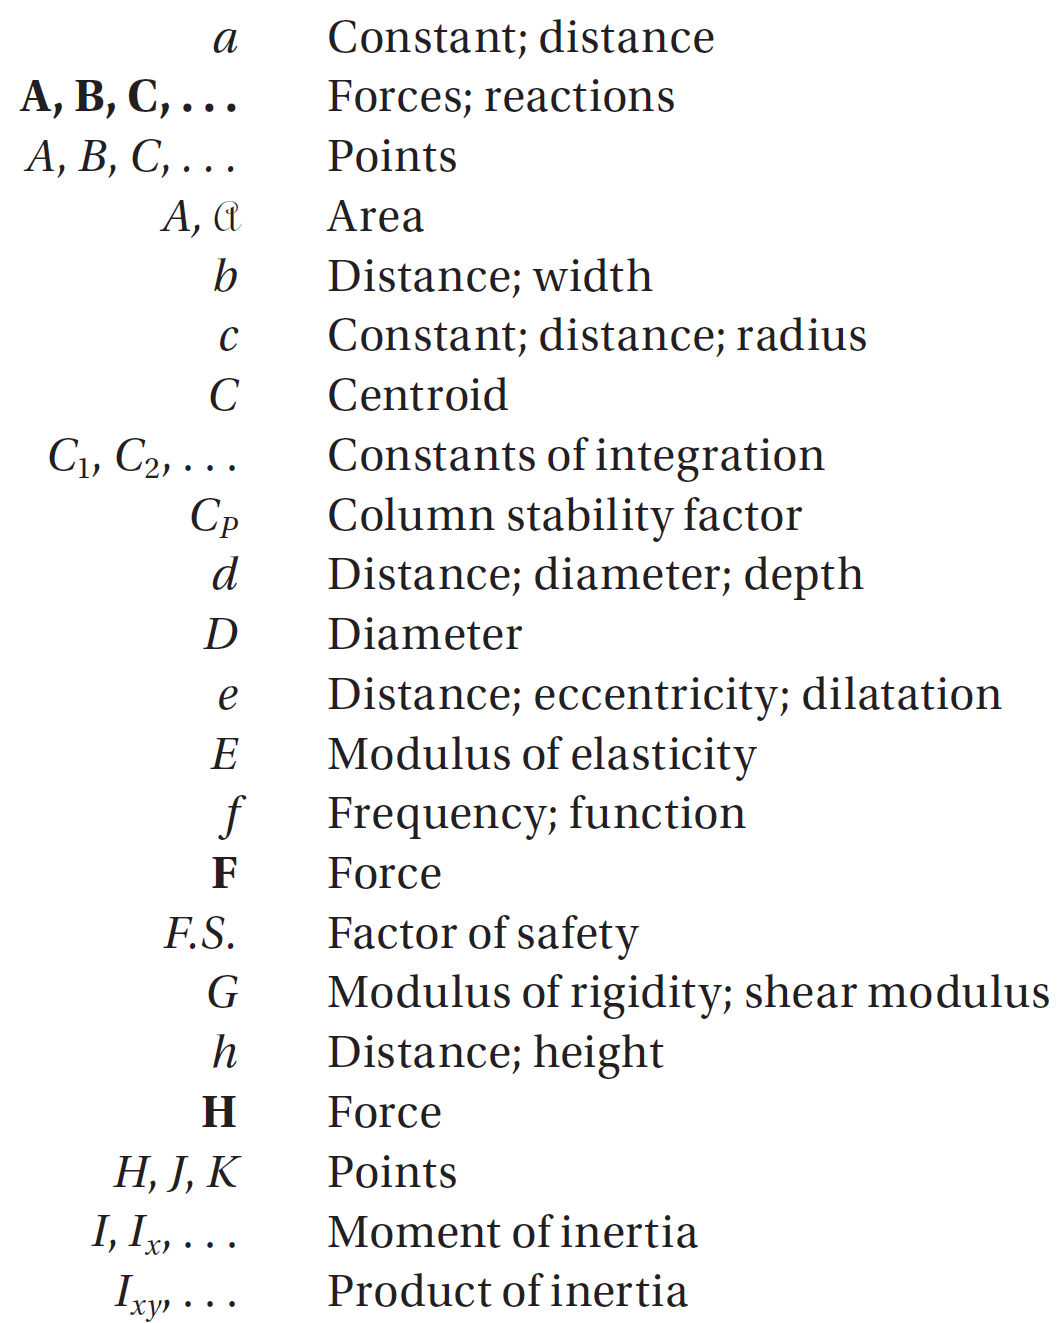
\includegraphics[width=\linewidth, height=8cm]{ListOfSymbols_Part_1.png}
\end{Figure}
\begin{Figure}
    \centering
    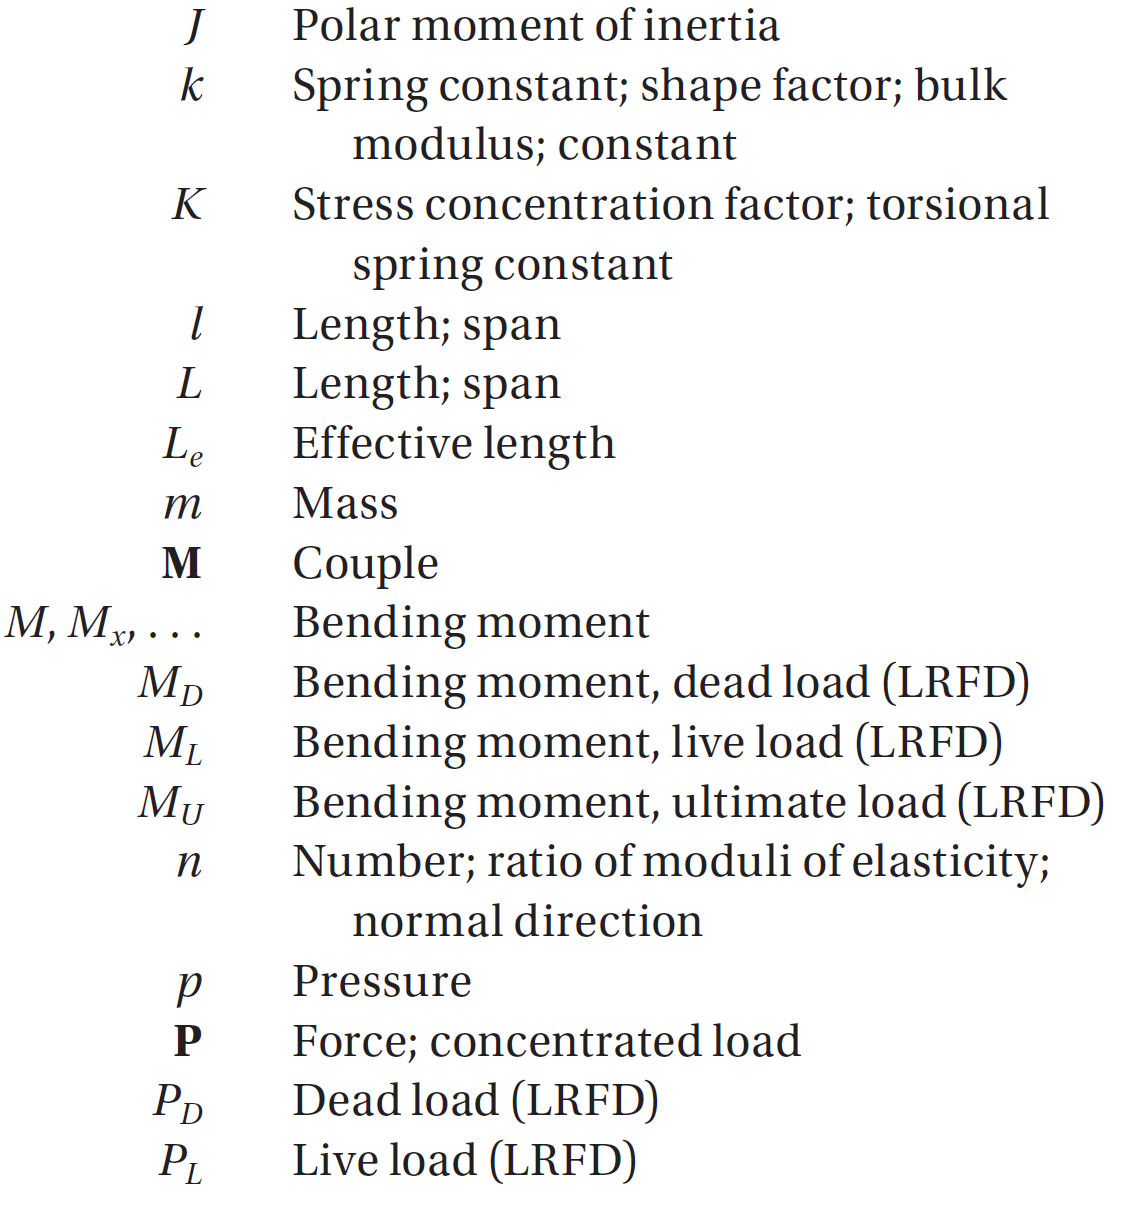
\includegraphics[width=\linewidth, height=8cm]{ListOfSymbols_Part_2.png}
\end{Figure}
\begin{Figure}
    \centering
    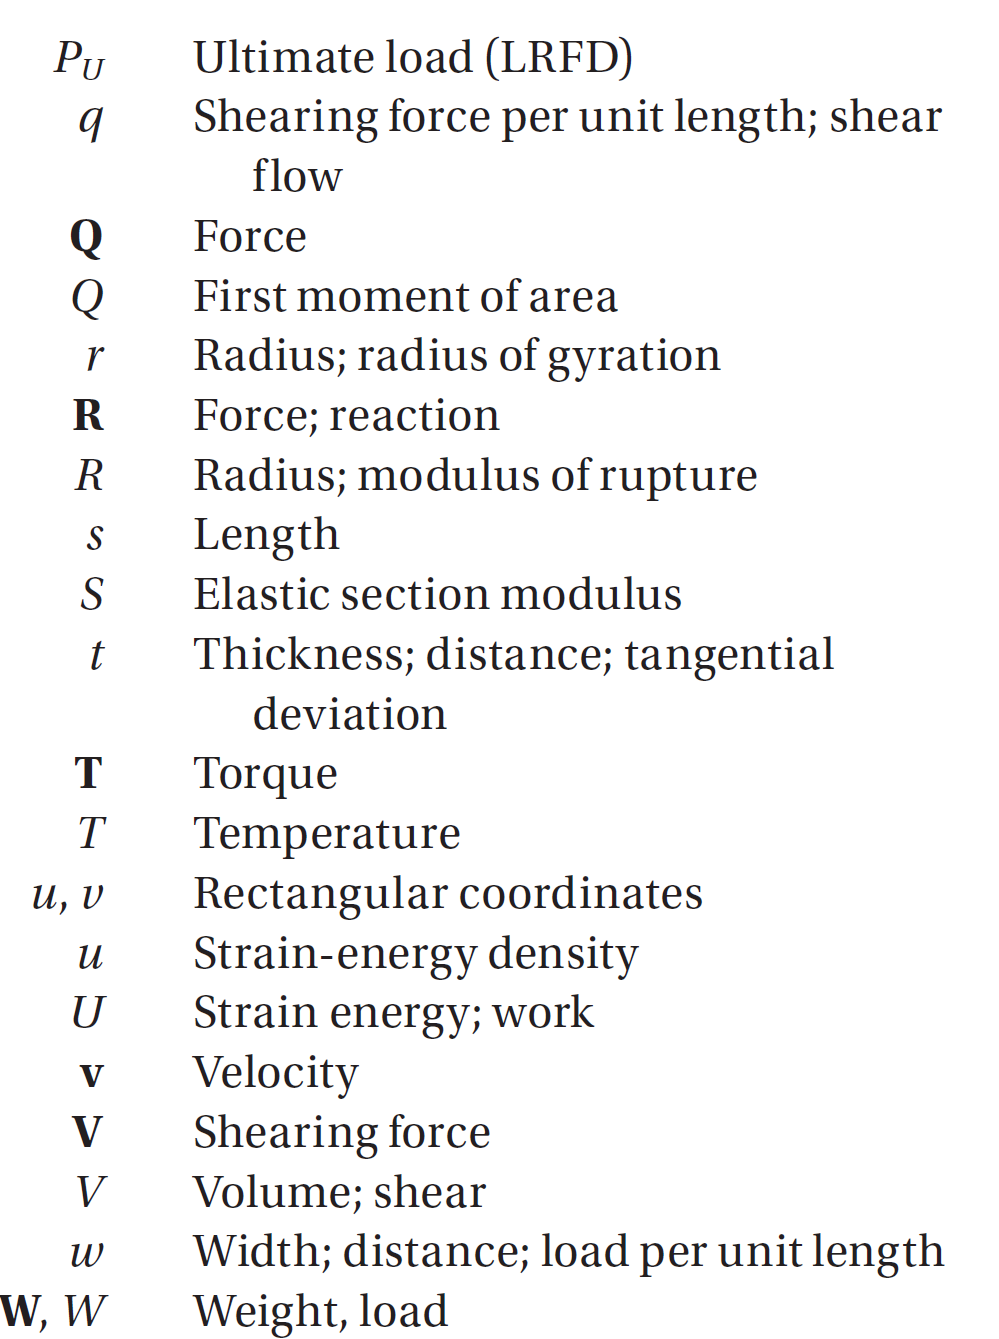
\includegraphics[width=\linewidth, height=8cm]{ListOfSymbols_Part_3.png}
\end{Figure}
\begin{Figure}
    \centering
    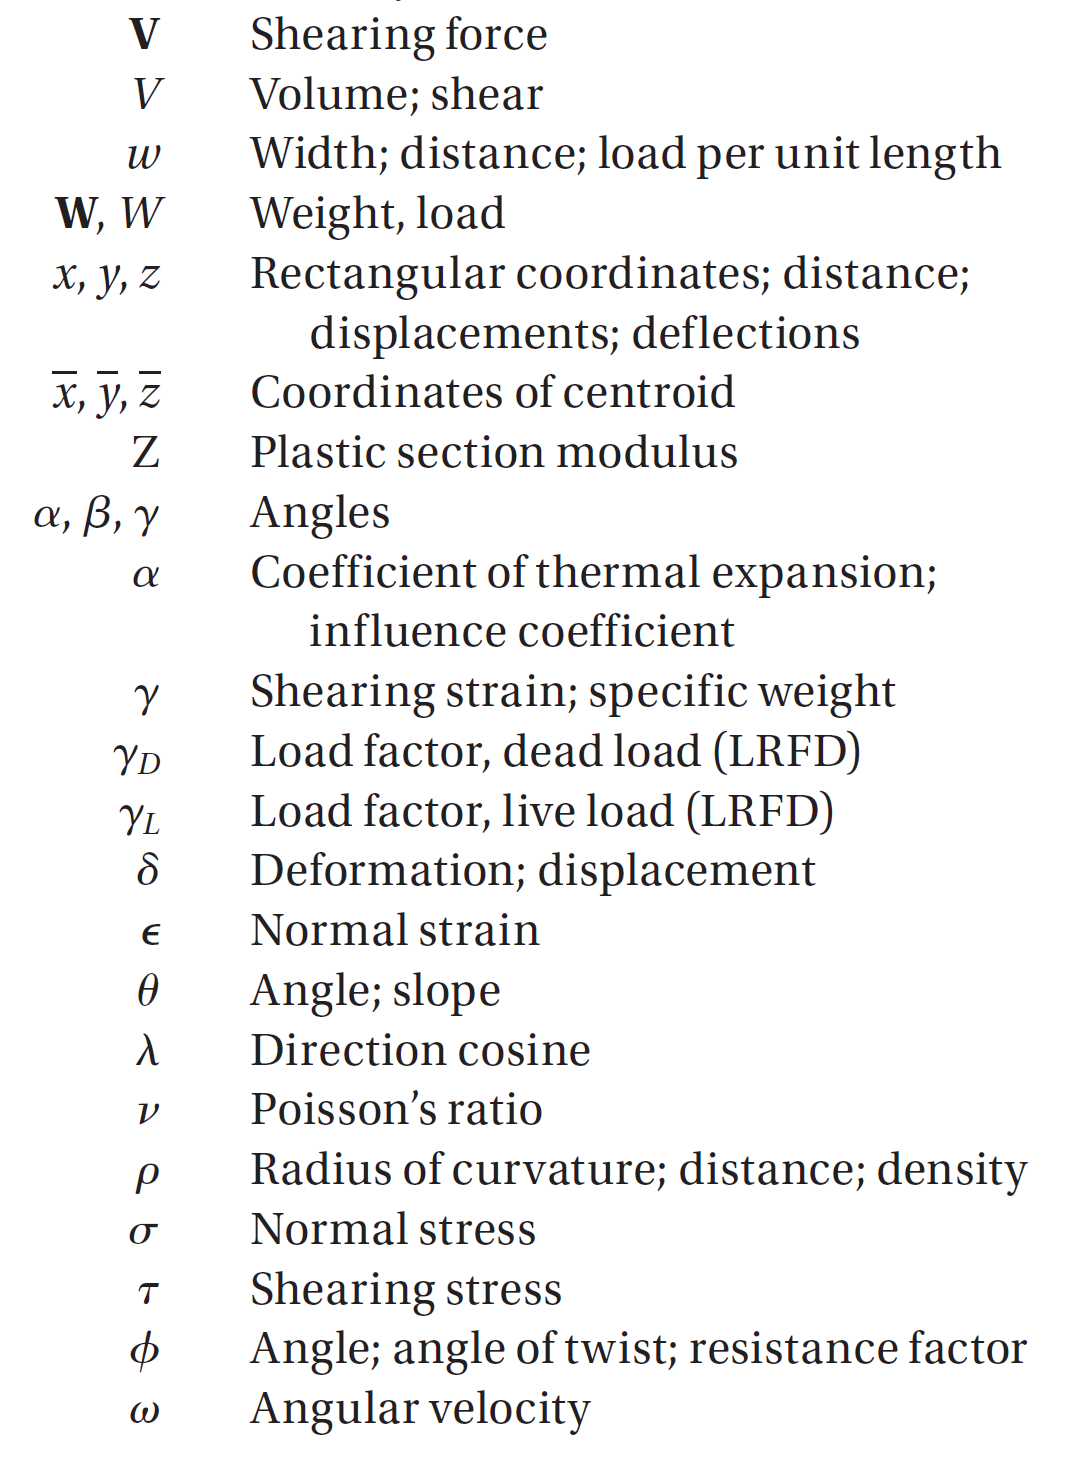
\includegraphics[width=\linewidth, height=10cm]{ListOfSymbols_Part_4.png}
\end{Figure}

\section{Conversion Factors}
\begin{equation}
    1\text{hp}=550\text{ft*lb/s}=6600\text{ in*lb/s}
\end{equation}

\section{General}
\begin{Figure}
    \centering
    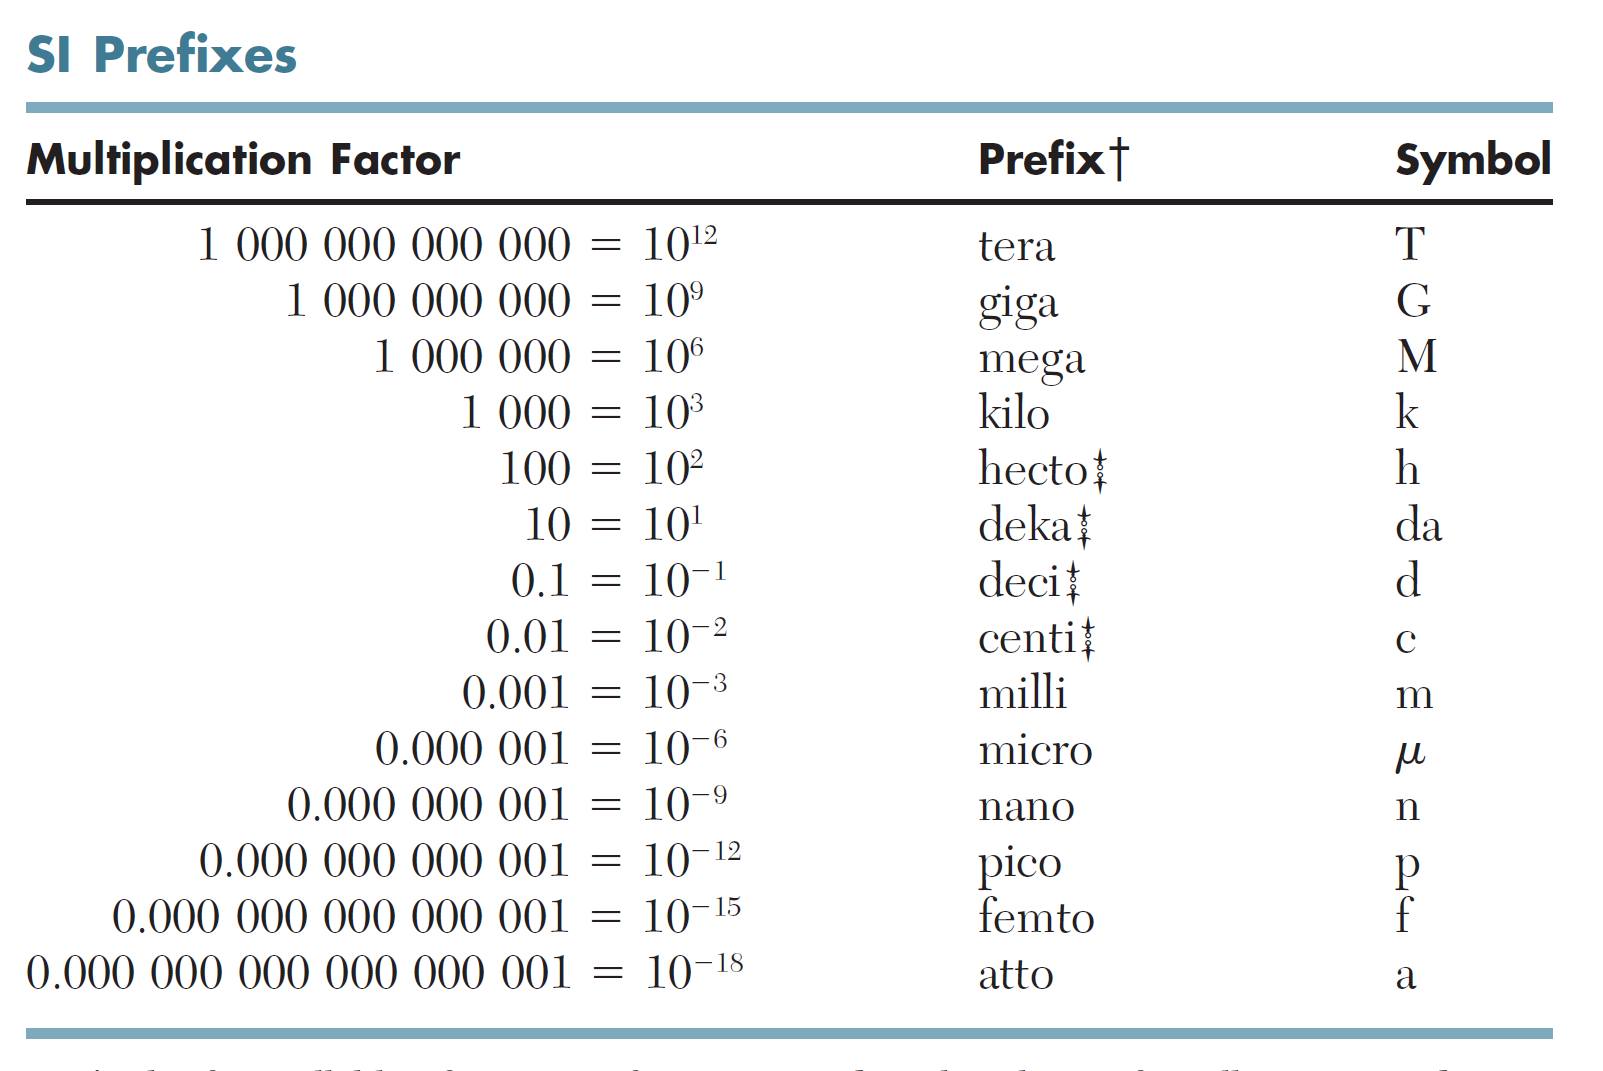
\includegraphics[width=\linewidth, height=8cm]{SI_Prefix.png}
\end{Figure}

\section{Moments}
\subsection{Moment of Inertia}
\subsubsection{Area Moment of Inertia for Rectangular Section}
\begin{equation}
    I_x=bh^3/12
\end{equation}
\subsection{Parallel Axis Theorm (2-Dimensional)}
\begin{equation}
    I=I_{\text{Original}}+Ad^2
\end{equation}

% -----------------------------------------------------------------------
\section{Chapter 1 - Concept of stress}
\subsection{Axial Loading: Normal Stress}
\begin{equation}
    \sigma=\frac{P}{A}
\end{equation}
\subsection{Transverse Forces and Shearing Stress}
\begin{equation}
    \tau_{\text{ave}}=\frac{P}{A}
\end{equation}
\subsection{Single and Double Shear}
\subsubsection{Single Shear}
\begin{equation}
    \tau_{\text{avg}}=\frac{P}{A}=\frac{F}{A}
\end{equation}
\subsubsection{Double Shear}
\begin{equation}
    \tau_{\text{avg}}=\frac{P}{A}=\frac{F/2}{A}=\frac{F}{2A}    
\end{equation}
\subsection{Bearing Stress}
\begin{equation}
    \sigma_b=\frac{P}{A}=\frac{P}{td}
\end{equation}
\subsection{Method of Solution}
\begin{enumerate}
  \item Clear and precise statement of problem
  \item Draw one or several free-body diagrams; used to write equilibrium equations
  \item Think SMART. Strategy, Modeling, Analysis, and Reflect \& Think
\end{enumerate}
\subsection{Stresses on an Oblique Section}
\begin{equation}
    \sigma=\frac{P}{A_0}cos^2\theta
\end{equation}
\begin{equation}
    \tau=\frac{P}{A_0}sin\theta cos\theta
\end{equation}
\section{Stress Under General Loading}
\section{Factor of Safety}
\begin{equation}
    \text{Factor of safety }=\text{ F.S. }=\frac{\text{ultimate load}}{\text{allowable load}}
\end{equation}

\section{Chapter 2 - Stress and Strain - Axial Loading}
\subsection{Normal Strain}
\begin{equation}
    \epsilon=\frac{\delta}{L}
\end{equation}
\subsection{Hooke's Law and Modulus of Elasticity}
\begin{equation}
    \sigma=E\epsilon
\end{equation}
\subsection{Elastic Deformation Under Axial Loading}
\begin{equation}
    \delta=\frac{PL}{AE}
\end{equation}
\begin{equation}
    \delta=\Sigma=\frac{P_iL_i}{A_iE_i}
\end{equation}
\subsection{Problems with Temperature Change}
\begin{equation}
    \delta_T=\alpha(\Delta T)L     
\end{equation}
\begin{equation}
    \epsilon_T=\alpha\Delta T
\end{equation}
\subsection{Lateral Strain and Poisson's Ratio}
\begin{equation}
    v=-\frac{\text{lateral strain}}{\text{axial strain}}
\end{equation}
\subsection{Multiaxial Loading}
\begin{equation}
    \epsilon_x=\frac{\sigma_x}{E}
\end{equation}
\begin{equation}
    \sigma_y=\sigma_x=-\frac{v\sigma_x}{E}
\end{equation}
\subsubsection{Generalized Hooke's law for multiaxial loading}
\begin{equation}
    \sigma_x=+\frac{\sigma_x}{E}-\frac{v\sigma_y}{E}-\frac{v\sigma_z}{E}
\end{equation}
\begin{equation}
    \sigma_y=-\frac{\sigma_x}{E}-\frac{v\sigma_y}{E}-\frac{v\sigma_z}{E}
\end{equation}
\begin{equation}
    \sigma_z=-\frac{\sigma_x}{E}-\frac{v\sigma_y}{E}+\frac{v\sigma_z}{E}
\end{equation}
\subsection{Dilation}
\begin{equation}
    e=\frac{1-2v}{E}(\sigma_x+\sigma_y+\sigma_z)
\end{equation}
\subsection{Bulk Modulus}
$p$: Hydrostatic Pressure
\begin{equation}
    e=-\frac{p}{k}
\end{equation}
$k$: bulk modulus of the material
\begin{equation}
    k=\frac{E}{3(1-2v)}
\end{equation}
\subsection{Shearing Strain: Modulus of Rigidity}
\begin{equation}
    \tau_{xy}=G\gamma_{xy}
\end{equation}
\begin{equation}
    \tau_{yz}=G\gamma{yz}
\end{equation}
\begin{equation}
    \tau_{zx}=G\gamma_{zx}
\end{equation}
\begin{equation}
    \frac{E}{2G}=1+v
\end{equation}
\subsection{Stress Concentrations}
\begin{equation}
    K=\frac{\sigma_\text{max}}{\sigma_\text{avg}}
\end{equation}

\section{Chapter 3 - Torsion}
\subsection{General}
\subsection{Deformation in Circular Shafts}
\begin{equation}
    \gamma=\frac{\rho\phi}{L}
\end{equation}
\begin{equation}
    \gamma_{max}=\frac{c\phi}{L}
\end{equation}
\begin{equation}
    \gamma=\frac{\rho}{c}*\gamma_{max}
\end{equation}
\subsection{Shearing Stresses in Elastic Range}
\begin{equation}
    \tau=\frac{\rho}{c}\tau_{max}
\end{equation}
\begin{equation}
    \tau_{max}=\frac{Tc}{J}
\end{equation}
\begin{equation}
    \tau=\frac{T\rho}{J}
\end{equation}
\subsubsection{Polar Moment of Inertia Solid Shaft}
\begin{equation}
    J=\frac{1}{2}\pi c^4
\end{equation}
c = radius
\subsubsection{Polar Moment of Inertia of a Hollow Shaft inner radius c1, outer radius c2}
\begin{equation}
    J=\frac{1}{2}\pi(c_2^4-c_2^4)
\end{equation}
\subsection{Angle of Twist}
\begin{equation}
    \phi=\frac{TL}{JG}
\end{equation}
\begin{equation}
    \phi=\Sigma\frac{TL}{JG}
\end{equation}
\subsection{Statically Indeterminante Shafts}
\subsection{Transmission Shafts}
Power P is transmitted as:
\begin{equation}
    P=2\pi fT
\end{equation}
T is the torque exerted at each end of the shaft\\*
f the frequency (hz or $s^{-1}$)
\subsection{Stress Concentrations}
\begin{equation}
    \tau_{\text{max}}=K\frac{Tc}{J}
\end{equation}
K = Stress concentration factor\\*
stress $\frac{Tc}{J}$ is computed for the smaller-diameter shaft
\begin{Figure}
    \centering
    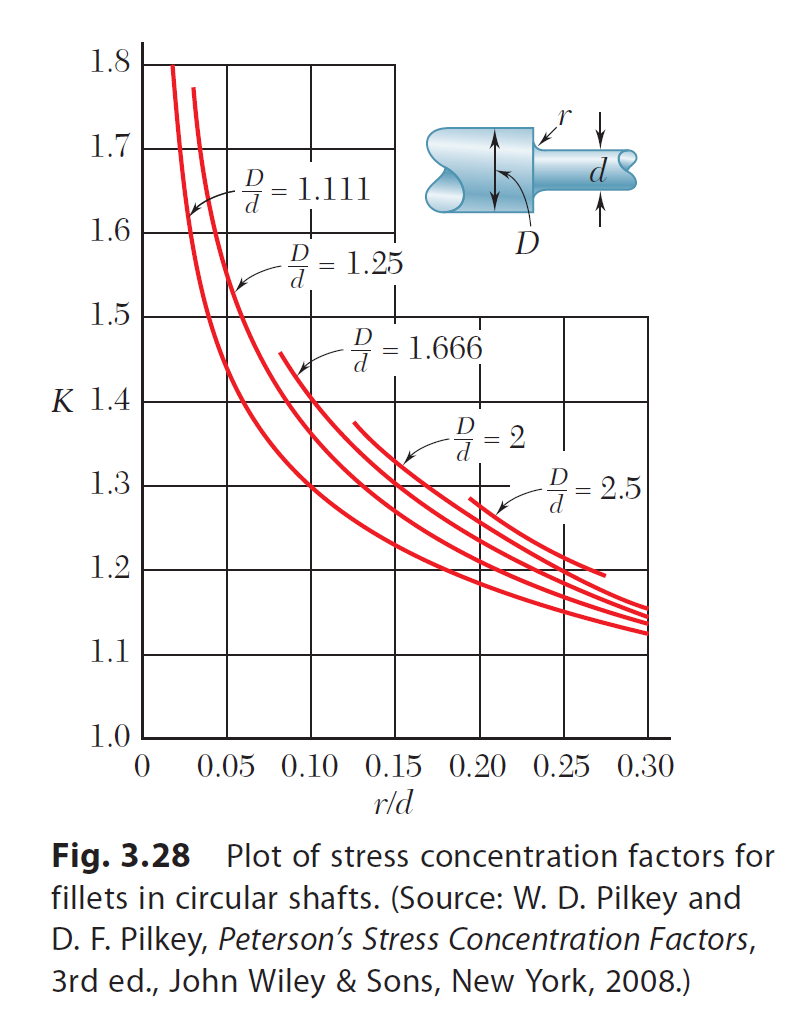
\includegraphics[width=\linewidth, height=8cm]{PlotStressConcentrationsFilletsRoundShaft.png}
\end{Figure}
\subsection{Plastic Deformations}
\begin{equation}
    T=\int^c_0\rho\tau(2\pi d\rho)=2\pi\int^c_0\rho^2\tau d\rho
\end{equation}
\subsection{Modulus of Rupture}
This is a ficticious value.
\begin{equation}
    R_t=\frac{T_uc}{j}
\end{equation}
\subsection{Solid Shaft of Elastoplastic Material}
\subsubsection{Maximum Elastic Torque; Solid Circular Shaft, Radius c}
\begin{equation}
    \tau_y=\frac{1}{2}\pi c^3\tau Y
\end{equation}
\subsubsection{Torque Related to $\rho_y$}
\begin{equation}
    T=\frac{4}{3}T_y(1-\frac{1}{4}\rho{\rho^3y}{c^3})
\end{equation}
\subsubsection{Plastic Torque}
\begin{equation}
    T_p=\frac{4}{3}T_y
\end{equation}
\subsubsection{Plastic Torque Vs. Angle of Twist}
\begin{equation}
    T=\frac{4}{3}T_y(1-\frac{1}{4}\frac{\phi^3y}{\phi^3})
\end{equation}
\subsubsection{Torsional Loading or Shaft Cross-Section Changes Along Length}
\begin{equation}
    \phi=\Sigma_i\frac{T_iL_i}{J_iG_i}
\end{equation}
\subsubsection{Thin-Walled Hollow Shafts}
\subsubsection{Shear Flow}
\begin{equation}
    q=\tau t
\end{equation}
\subsubsection{Average Shearing Stress $\tau$ at any given point in cross section}
\begin{equation}
    \tau=\frac{T}{2tA}
\end{equation}

\section{Chapter 4 - Pure Bending}
\subsection{1 - Symmetric Members in Pure Bending}
\begin{equation}
    \epsilon_x=-\frac{y}{\rho}
\end{equation}
$\rho$ - Radius of curvature of the neutral surface\\*
$y$ - Distance from neutral surface
\subsection{2 - Stresses and Deformatoins in the Elastic Range}
\begin{equation}
    \sigma_x=-\frac{y}{c}\sigma_m
\end{equation}
c - largest distance from the neutral axis to a point in the section\\*
\subsubsection{Elastic Flexture formula}
\begin{equation}
    \sigma_m=\frac{Mc}{I}
\end{equation}
Equation To Use When Finding Normal Internal Stress
\begin{equation}
    \sigma_x=-\frac{My}{I}
\end{equation}
$-\sigma$ -- Compression\\*
 $\sigma$ -- Tension
\subsubsection{Eleastic Section Modulus}
\begin{equation}
    S=\frac{I}{c}
\end{equation}
\begin{equation}
    \sigma_m=\frac{M}{S}
\end{equation}
\subsubsection{Curvature of Member}
\begin{equation}
    \frac{1}{\rho}=\frac{M}{EI}
\end{equation}
\subsection{Eccentric Axial Loading}
\begin{equation}
    \sigma_x=\frac{P}{A}-\frac{M_y}{I}    
\end{equation}
\subsection{Unsymmetric Bending}
\begin{equation}
    \sigma_x=-\frac{M_zy}{I_z}+\frac{M_yz}{I_y}
\end{equation}
\subsection{General Eccentric Axial Loading}
\begin{equation}
    \sigma_x=\frac{P}{A}-\frac{M_zy}{I_z}+\frac{M_yZ}{I_y}
\end{equation}
\subsection{Curved Members}
\begin{equation}
    R=\frac{A}{\int\frac{dA}{r}}
\end{equation}
\begin{equation}
    \sigma_x=-\frac{My}{Ae(R-y)}
\end{equation}
\subsection{Factor of Safety}
\begin{equation}
    \sigma_m=K\frac{Mc}{I}
\end{equation}
\begin{Figure}
    \centering
    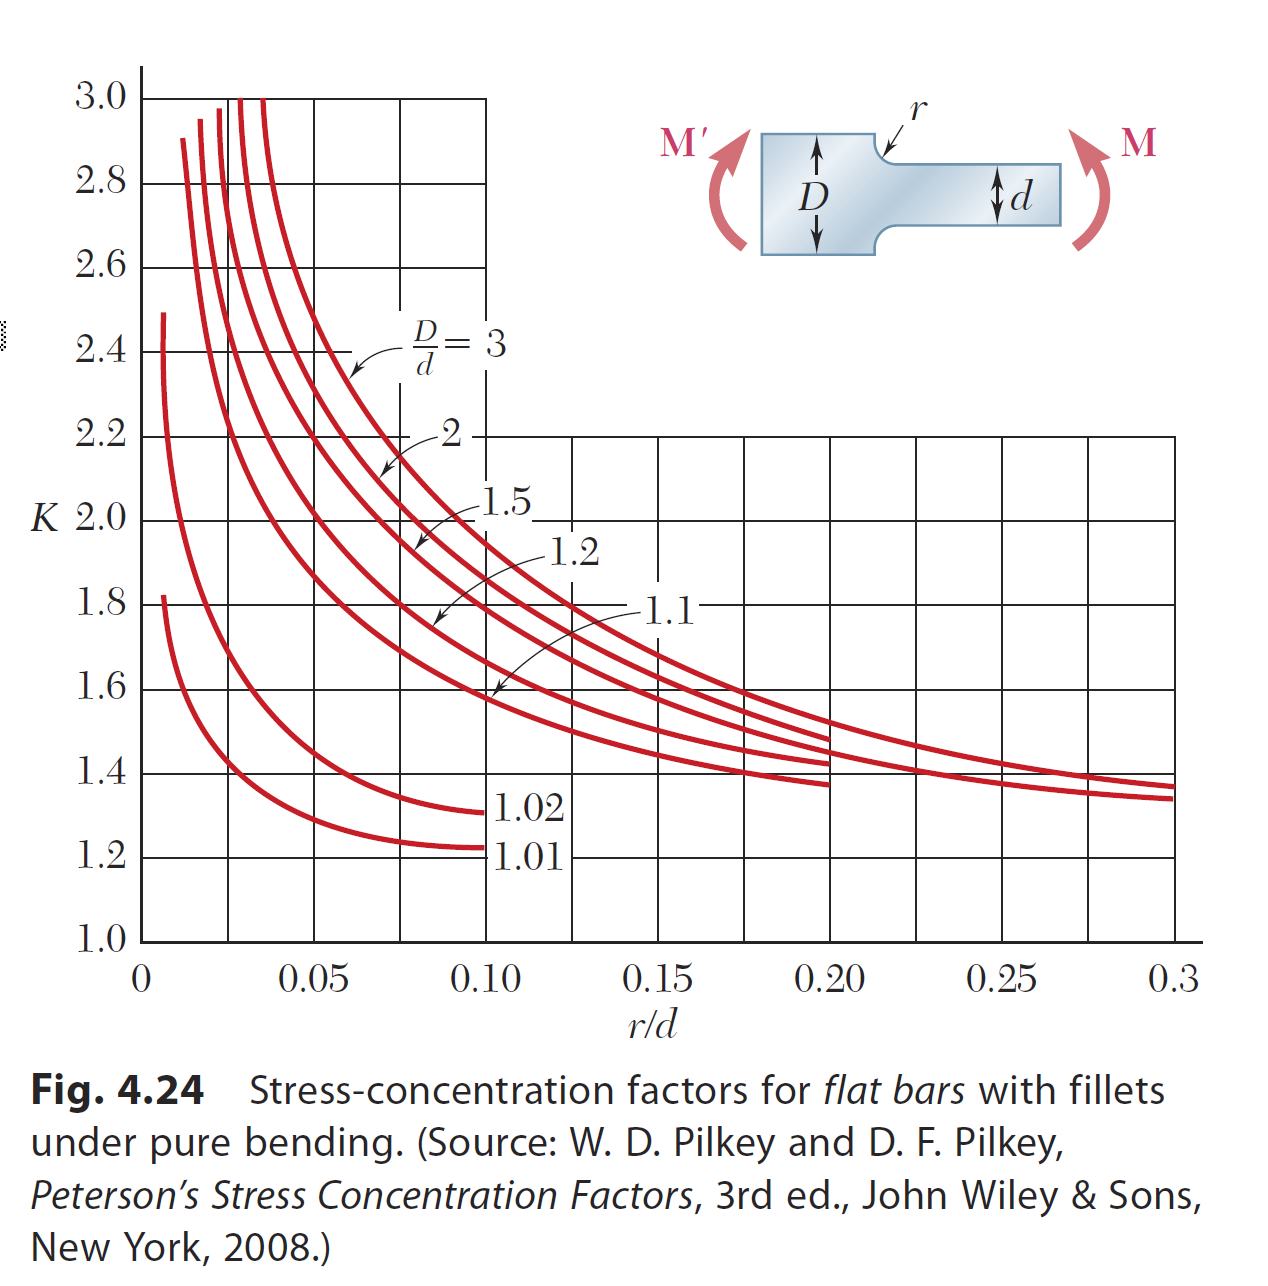
\includegraphics[width=\linewidth]{Fig_4_24.png}
\end{Figure}
\begin{Figure}
    \centering
    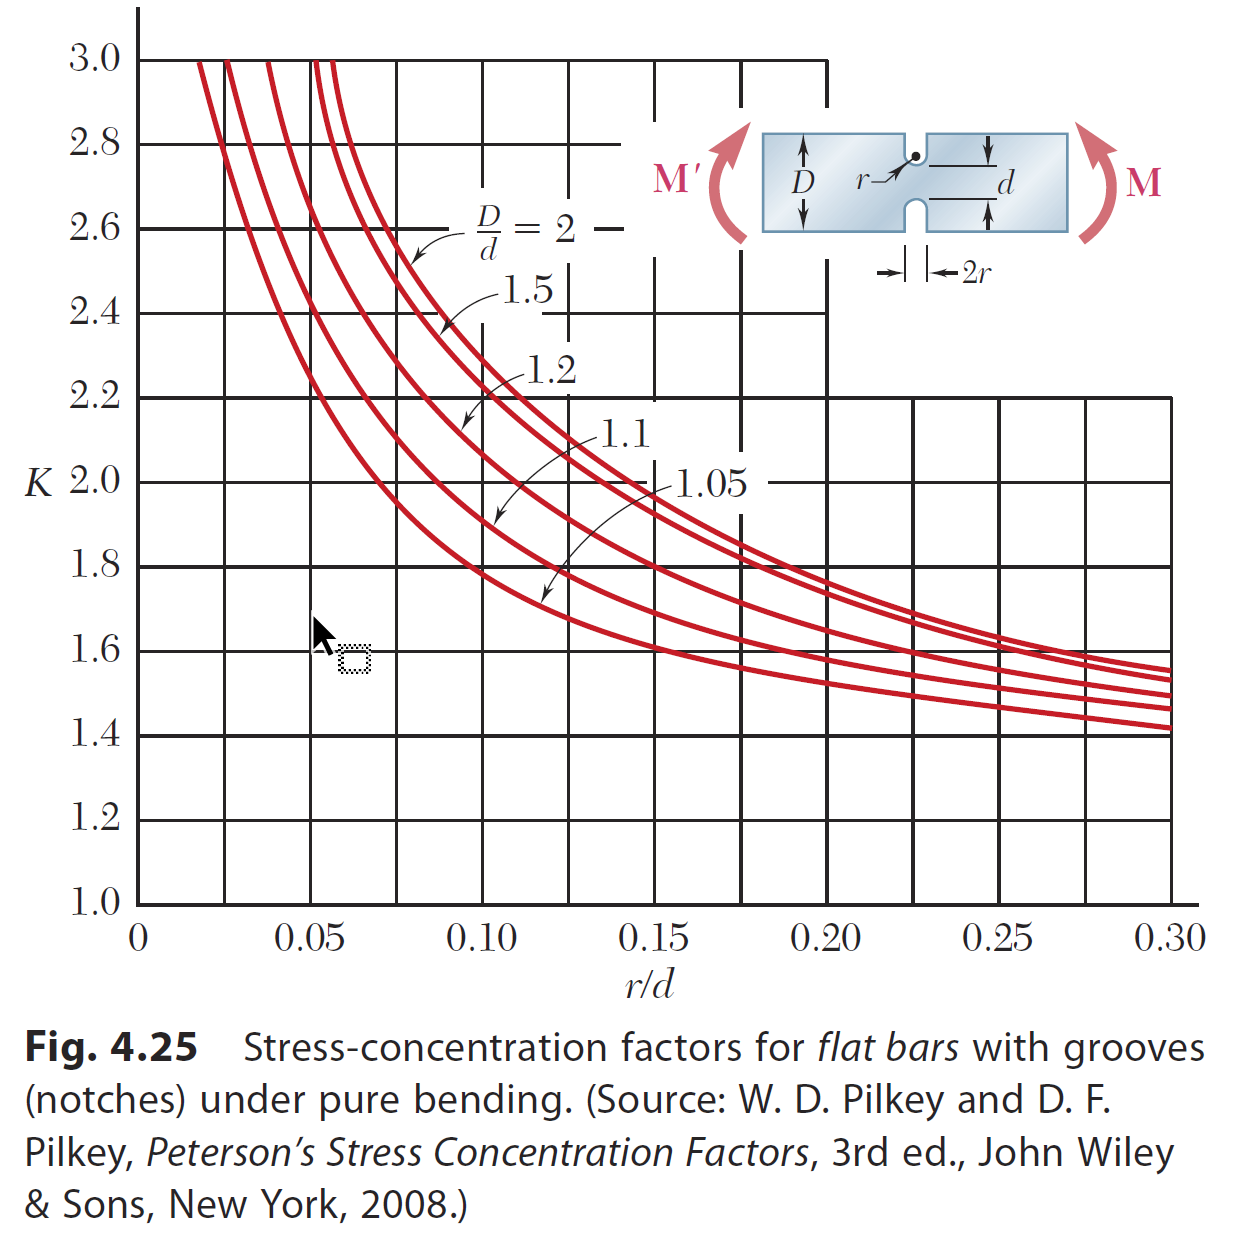
\includegraphics[width=\linewidth]{Fig_4_25.png}
\end{Figure}
\subsubsection{Equation for Force on a Single Area Within a T Section}
\begin{equation}
    F=\int dF=-\int\frac{My}{I}dA=-\frac{M}{I}\int ydA=-\frac{M}{I}\bar{y}*A*
\end{equation}
\subsection{Additional Notes}
Area, width, and moment of inertia for W shapes should be given on a test or found in appendix c of textbook.\\*
c in this section is the largest distance from the neutral axis to a point in the section.
%\subsection{3 - Deformations in a Transverse Cross Section}
%\subsection{4 - Members Made of Composite Materials}
%\subsection{5 - Stress Concentrations}
%\subsection{6 - Plastic Deformations}
%\subsection{7 - Eccentric Axial Loading in a Plane of Symmetry}
%\subsection{8 - Unsymmetric Bending Analysis}
%\subsection{9 - General Case of Eccentric Axial Loading Analysis}
%\subsection{10 - Curved Members}

% Example Figure
%\begin{Figure}
%    \centering
%    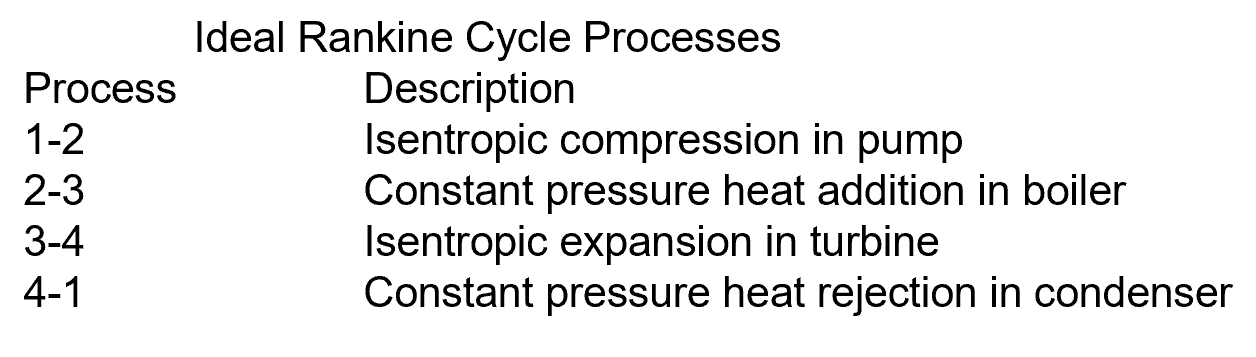
\includegraphics[width=\linewidth]{RankineCycleProcess.png}
%\end{Figure}

% References
%\rule{0.3\linewidth}{0.25pt}
%\scriptsize
%\bibliographystyle{abstract}
%\bibliography{Bibliography}

% End of document
\end{multicols}
\end{document}